\documentclass{article}
\usepackage[utf8]{inputenc}
\usepackage{amsthm}
\usepackage{amsmath}
\usepackage{amssymb}
\usepackage{enumitem}
\usepackage{float}
\usepackage{graphicx}
\setlength{\parindent}{0em}
\setlength{\parskip}{1em}
\usepackage{fixltx2e}
\newcommand{\Mod}[1]{\ (\mathrm{mod}\ #1)}
\usepackage{mathabx}
\DeclareMathOperator{\tr}{tr}
\usepackage{geometry}
\graphicspath{ {./graphics/} }
 \geometry{
 a4paper,
 total={170mm,257mm},
 left=20mm,
 top=20mm,
 }

\newenvironment{QandA}{\begin{enumerate}[label=\bfseries\alph*.]\bfseries}
                      {\end{enumerate}}
\newenvironment{answered}{\par\normalfont}{}

\title{Calculus 18/19 Sem 1 Suggested Answers}

\author{\makebox[.9\textwidth]{NUS LaTeXify Proj Team}}
\date{Updated: 28 December 2019}

\begin{document}

\maketitle
Done by: Yip Jung Hon and Pan Jing Bin
\hline

\subsubsection*{Question 1}
\begin{enumerate}[label=\roman*)]
\item
Let $\epsilon > 0$. Choose $\delta=\min\{1/2,\epsilon/6 \}$.\\
Then whenever $0<|x-2|<\delta$:
\begin{align*}
    \left|\frac{2x^2+3x+1}{x^2-1}-5\right| &= \left|\frac{2x^2+3x+1-5x^2+5}{x^2-1}\right|\\
    &=\left|\frac{-3x^2+3x+6}{x^2-1}\right|\\
    &=3\left|\frac{(x-2)(x+1)}{(x-1)(x+1)}\right|\\
    &=3\left|\frac{x-2}{x-1}\right|\\
    &<3\left|\frac{\delta}{\frac{1}{2}}\right|\\
    &=6\delta\\
    &< \epsilon
\end{align*}
\item Consider 2 cases:

Case 1: If $f(0)=0$ or $f(1)=1$, then it definitely cuts the line $y=x$ at either $x=0$ or $x=1$.

Case 2: $f(0)\neq0$ and $f(1)\neq1$. We define $g(x)=f(x)-x$. Then $g$ is continuous on $(0,1)$.
\begin{flalign*}
f(0)\neq0\implies f(0)>0\implies g(0)>0 \\
f(1)\neq1\implies f(1)<1\implies g(1)<0 &&
\end{flalign*}
Since $g(0)>0$ and $g(1)<0$ and $g$ is continuous on $[0,1]$, by the IVT, $\exists c\in(0,1)$ such that $g(c)=0 \implies f(c)=c$.
\end{enumerate}

\pagebreak
\subsubsection*{Question 2}

\begin{enumerate}[label=\roman*)]
    \item Given $f(x+y)=f(x)+f(y)+x^2y+xy^2$.
        \begin{flalign}
            f'(x)&=\lim_{h \rightarrow 0} \frac{f(x+h)-f(x)}{h} \nonumber\\
            &=\lim_{h \rightarrow 0} \frac{f(x)+f(h)+x^2h+xh^2-f(x)}{h} \nonumber \\
            &= \lim_{h \rightarrow 0} \frac{f(h)}{h} + x^2 + xh \nonumber \\
            &= x^2+1&&
        \end{flalign}
    Taking the derivative at $0$, we have $f'(0)=1$, however, 
    \begin{flalign*}
        f'(0)=1=&=\lim_{x \rightarrow 0} \frac{f(x)-f(0)}{x-0}\\
        &=\lim_{x \rightarrow 0} \frac{f(x)}{x} - \frac{f(0)}{x} \\
        &= 1 - \lim_{x \rightarrow 0} \frac{f(0)}{x}&&
    \end{flalign*}
    If $f(0)$ was not 0, then one would have $\lim_{x \rightarrow 0} \frac{f(0)}{x}$ going to infinity, which is a contradiction. Thus $f(0)=0$. Integrating (1), $f(x)=\frac{1}{3}x^3+x+c$. Subbing $f(0)=0$, we have that $c=0$, and hence $f(x)=\frac{1}{3}x^3+x$.
    
    \item $\lim_{x \rightarrow 0} \frac{(ax+b)^{1/3}-2}{x}=5/12$.
    Note that this implies that numerator must go to 0, as else if it approached some value greater than 0, it would mean the integral would go off to infinity. Solving for $\lim_{x \rightarrow 0}(ax+b)^{1/3}-2=0$, we find that $\lim_{x \rightarrow 0}ax+b=8 \implies b=8$.
    
    Since both the numerator and denominator go to 0, we can apply L'Hopital's Rule:
    \begin{align*}
        \lim_{x \rightarrow 0} \frac{(ax+b)^{1/3}-2}{x} &= \lim_{x \rightarrow 0} \frac{a}{3}(ax+8)^{-2/3} \\
        &=\frac{a}{3}(8^{-2/3})=5/12
    \end{align*}
    Solving, $a=5, b=8$.
    
    \item If $f(x)=\frac{x^27+x^26+2}{1+x}$, evaluate $f^{27}(x)$.
    By polynomial long division, we have $f(x)=x^{26}+\frac{2}{x+1}$. Differenciating $f$ 27 times will make the $x^{26}$ term disappear, so we only need to worry about the $\frac{2}{x+1}$ term. Note that if $g(x)=\frac{2}{x+1}$, then $g^1(x)=-\frac{2}{(x+1)^2}, g^2(x)=\frac{2 \times 2}{(x+1)^3}, g^3(x)=-\frac{2 \times 2 \times 3}{(x+1)^4}$. In general, we realise that:
    \begin{align*}
        &g^n(x)=(-1)^n \frac{2n!}{(x+1)^n+1} \\
        &g^{27}(3) = -\frac{2 \times 27!}{4^{28}}
    \end{align*}
\end{enumerate}

\pagebreak
\subsubsection*{Question 3}
\begin{enumerate}[label=\roman*)]
\item Applying implicit differentiation:
\begin{align*}
    &2x+y+x\frac{dy}{dx}+2y\frac{dy}{dx}=0\\
    &\frac{dy}{dx}(x+2y)=-2x-y\\
    &\frac{dy}{dx}=\frac{-2x-y}{x+2y}\\
\end{align*}
$dy/dx$ is undefined at $x=-2y$. $dy/dx=0\implies x=-y/2$.
At $x=-2y$:
\begin{align*}
    &(-2y)^2+(-2y)y+y^2=12\\
    &4y^2-2y^2+y^2=12\\
    &3y^2=12\\
    &y=\pm 2
\end{align*}
We also need to check the point where by $dy/dx$ is undefined. At $x=-y/2$:
\begin{align*}
    &(-\frac{y}{2})^2+(-\frac{y}{2})y+y^2=12\\
    &\frac{y^2}{4}-\frac{y^2}{2}+y^2=12\\
    &y^2=16\\
    &y=\pm 4
\end{align*}
We have $4$ critical points: $(-4,2),(4,-2),(-2,4),(2,-4)$.

Highest point: $(-2,4)$. Lowest point: $(2,-4)$.
\item The curve $y=cx^3+e^x$ is continuous on $\mathbb{R}$.
\begin{align*}
    &y=cx^3+e^x\\
    &\frac{dy}{dx}=3cx^2+e^x\\
    &\frac{d^2y}{dx^2}=6cx+e^x
\intertext{Note that $\forall c\in\mathbb{R}$:}
    &\lim_{x\to+\infty} \frac{d^2y}{dx^2} = +\infty
\end{align*}
Thus the curve have inflection points if $\exists d\in\mathbb{R}$ such that $6c(d)+e^d <0$. (If such d exists, the intermediate value theorem will ensure that there exist a point where $\frac{d^2y}{dx^2}=0$).

Consider 3 cases: 

Case 1: $c>0$.
\begin{align*}
    &\lim_{x\to-\infty} \frac{d^2y}{dx^2} = -\infty
\intertext{Thus if $c>0$,the curve will have inflection points.}
\intertext{Case 2: $c<0$.}
    &\frac{d^3y}{dx^3}=6c+e^x\\
    &\frac{d^3y}{dx^3}=0\implies 6c=-e^x \implies x=\ln{-6c}\\ 
\intertext{$\frac{d^2y}{dx^2}$ has a local minimum at $x = \ln{-6c}$,}
    &6c(\ln{-6c})+e^{\ln{-6c}}<0\\
    &6c(\ln{-6c})<6c\\
    &\ln{-6c}>1\ \ \text{(Since $6c<0$)}\\
    &-6c>e\\
    &c<-\frac{e}{6}
\end{align*}
Case 3: $c=0$.

$e^x>0\implies \frac{d^2y}{dx^2}>0$ thus the curve does not have inflection points.

Combining the 3 cases, we have $c>0$ or $c<-\frac{e}{6}$.
\item There are two ways of doing this. One way is to simply recall the definition of $e^a$ as:
\begin{align*}
    e^a&=\lim_{x\to\infty} \left(1+\frac{a}{x}\right)^x \\
\intertext{Then we simplify the given expression to see:}
    \lim_{x\to\infty} \left(\frac{x+a}{x-a}\right)^x &= \lim_{x\to\infty} \left(1+\frac{2a}{x-a}\right)^x = e^{2a} \\
\intertext{Another way is to calculate limits by exponentiation: }
    \lim_{x\to\infty} \left(\frac{x+a}{x-a}\right)^x &=\lim_{x\to\infty} e^{x\ln{\frac{x+a}{x-a}}}\\
    \lim_{x\to\infty}x\ln{\frac{x+a}{x-a}}&=\lim_{x\to\infty}\frac{\ln{\frac{x+a}{x-a}}}{x^{-1}}\\
    \intertext{Since the top and bottom goes to 0, we can use L'Hopital's Rule.}
    &=\lim_{x\to\infty}\frac{\frac{(x-a)^{-1}+(x+a)(-1)(x-a)^{-2}}{\frac{x+a}{x-a}}}{-x^{-2}}\\
    &=\lim_{x\to\infty}\frac{\frac{(x-a)-(x+a)}{(x+a)(x-a)}}{-x^{-2}}\\
    &=\lim_{x\to\infty}\frac{2ax^2}{(x^2-a^2)}\\
    &=\lim_{x\to\infty}\frac{2a}{1-\frac{a^2}{x^2}}\\
    &=2a
\intertext{Comparing the powers, we see that $a=1/2$.}
    &e^{2a} = e \implies a=\frac{1}{2}
\end{align*}
\end{enumerate}
\pagebreak


\subsubsection*{Question 4}
\begin{enumerate}[label=\alph*)]
    \item Let the 2 points which the curve cuts $c$ be $c_1$ and $c_2$, where $c_2 > c_1$.
    
    \begin{figure}[H]
        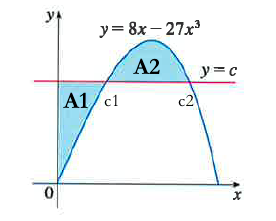
\includegraphics[width=6cm]{qn4a.png}
        \centering
    \end{figure}
    \begin{flalign*}
        A_1 = cc_1 - \int^{c_1}_0 8x-27x^3 dx \hspace{25pt} 
        A_2 = \int^{c_2}_{c_1}8x-27x^3 dx - c[c_2-c_1]
    \end{flalign*}
    Equating:
    \begin{align*}
        &cc_1 - \int^{c_1}_0 8x-27x^3 dx = \int^{c_2}_{c_1}8x-27x^3 dx - cc_2+cc_1 \\
        &cc_2=\int^{c_2}_0 8x-27x^3 dx \\
        &cc_2=4x^2-\frac{27}{4}x^4\Big|^{c_2}_0 \\
        &cc_2=4c_2^2-\frac{27}{4}c_2^4 \\
        &c=4c_2-\frac{27}{4}c_2^3 
    \intertext{Since $c_2$ is also a solution to $y=8x-27x^3, c=8c_2-27c_2^3$.}
        &8c_2-27c_2^3=4c_2-\frac{27}{4}c_2^3 \\
        &4=\frac{81}{4}c_2^2 \\
        &c_2 = \frac{4}{9} \ \ \text{(Reject -ve)} 
    \end{align*}
    We have $c=32/27$.
    \item We need to evaluate the integral $\int_0^1 2\pi(4-x^2)\sqrt{1+4x^2}\ dx$.
    
    For this question, we apply the integral reduction formula for $\sec^nx$.
    \begin{equation*}
        I_n=\int\sec^n(x)dx=\frac{1}{n-1}(\sec^{n-2}x\tan x)+\frac{n-2}{n-1}I_{n-2}+C
    \end{equation*}
    Letting $x=\tan u/2$, then $dx/du=\sec^2u/2$.
    \begin{align*}
        \int_0^1 2\pi(4-x^2)\sqrt{1+4x^2}\ dx &=\int^{\tan^{-1}2}_0 2\pi(4-\frac{1}{4}\tan^2u\sqrt{1+\tan^2u}\frac{1}{2}\sec^2u du
        \\
        &=\frac{1}{4}\pi \int^{\tan^{-1}2}_0 (16-\tan^2u)(\sec^3u)du \\
        &=\frac{\pi}{4} \int^{\tan^{-1}2}_0 (17\sec^3u-\sec^5u) du
    \end{align*}
    Apply integral reduction on $\sec^5u$, one has:
    \begin{align*}
        \int^{\tan^{-1}2}_0 \sec^5udu &= \frac{\tan u \sec^3u}{4}\Big|^{\tan^{-1}2}_0+\frac{3}{4}\int^{\tan^{-1}2}_0 \sec^3u du\\
    \end{align*}
    Considering a triangle: 
        \begin{figure}[H]
            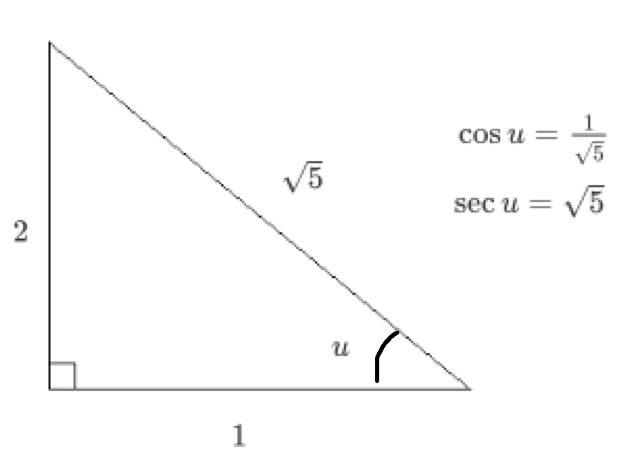
\includegraphics[width=6cm]{qn4b.png}
            \centering
        \end{figure}
    \begin{align}
        \frac{\tan[\tan^{-1}(2)]5\sqrt{5}}{4}+\frac34\int^{\tan^{-1}2}_0 \sec^3u du=\frac{5\sqrt{5}}{2}+\frac34\int^{\tan^{-1}2}_0 \sec^3u du
    \end{align}
    Due to (2), the integral reduces to:
    \begin{align}
        \frac{\pi}{4} \int^{\tan^{-1}2}_0 (17\sec^3u-\sec^5u) du&=-\frac{\pi}{4}\frac{5\sqrt{5}}{2} + \frac{\pi}{4}\int^{\tan^{-1}2}_0 \left(\frac{65}{4}\sec^3u\right) du
    \end{align}
    Apply integral reduction on $\sec^3u$, one has:
    \begin{align*}
        \int^{\tan^{-1}2}_0 \sec^3udu &= \frac{\tan u \sec u}{2}\Big|^{\tan^{-1}2}_0+\frac{1}{2}\int^{\tan^{-1}2}_0 \sec u du\\
        &=\sqrt{5} + \frac{1}{2} \ln(\sec x + \tan x) \big|^{\tan^{-1}2}_0 \\
        &=\sqrt{5} + \frac{1}{2}(\ln(\sqrt 5 + 2) - \ln(1)) \\
        &=\sqrt{5} + \frac{1}{2}(\ln(\sqrt 5 + 2))
    \end{align*}
    Going back to (3), we have:
    \begin{align*}
        -\frac{\pi}{4}\frac{5\sqrt{5}}{2} +\frac{\pi}{4}\int^{\tan^{-1}2}_0 \left(\frac{65}{4}\sec^3u\right) du &=
        -\frac{\pi}{4}\frac{5\sqrt{5}}{2} +
        \frac{65\pi}{16} (\sqrt{5} + \frac{1}{2}(\ln(\sqrt 5 + 2)))\\
        &\approx 33.4
    \end{align*}
\end{enumerate}

\pagebreak
\subsubsection*{Question 5}
\begin{enumerate}[label=\roman*)]
\item We have to split and evaluate the integral first.
\begin{align*}
    f(x)&=\int^\pi_0 (\cos{t})\cos{(x-t)}dt\\
    &=\int^\pi_0(\cos{t})(\cos{x}\cos{t}+\sin{x}\sin{t})dt\\
    &=\cos{x}\int^\pi_0\cos{^2t}dt + \sin{x}\int^\pi_0 \sin{t}\cos{t}dt\\
    &=\cos{x}\int^\pi_0\frac{1}{2}\cos{2t}+\frac{1}{2}dt+\sin{x}\int^\pi_0\frac{1}{2}\sin{2t}dt\\
    &=\cos{x}\left[\frac{1}{4}\sin{2t}+\frac{t}{2}\right]^\pi_0 - \sin{x}\left[\frac{1}{4}\cos{2t}\right]^\pi_0\\
    &=\cos{x}(\frac{\pi}{2})-\sin{x}(0)\\
    &=\frac{\pi}{2}\cos{x}\\
    f'(x)&=-\frac{\pi}{2}\sin{x}
\end{align*}

$f'(x)=0\implies \sin{x}=0\implies x=0,x=\pi,x=2\pi$.

$f(0)=\frac{\pi}{2}$, $f(\pi)=-\frac{\pi}{2}$, $f(2\pi)=\frac{\pi}{2}$.

Thus the minimum of $f(x)$ on $[0,2\pi]$ is $(\pi,-\frac{\pi}{2})$.

\item We prove this by strong induction. Let $P(n)$ be the predicate: $\int^1_0(\ln{x})^ndx=(-1)^n\cdot n!$\\\\
Base case($n=0$ and $n=1$):
\begin{align*}
    &\int^1_0(\ln{x})^0dx = \int^1_0 1 dx= 1\\
    &(-1)^0\cdot(0!) = 1 =\int^1_0(\ln{x})^0dx
\intertext{Thus $P(0)$ is true.}
    &\int^1_0\ln{x}dx = [x\ln{x}-x]\big|^1_0 = -1\\
    &(-1)^1\cdot(1!)=-1=\int^1_0\ln{x}dx \\
\intertext{Thus $P(1)$ is true.}
\intertext{Inductive step: Assume $P(n), P(n-1) \ldots P(0)$ is true, to show $P(n+1)$ is true.}
    \int^1_0(\ln{x})^{n+1}dx &= \int^1_0(\ln{x})(\ln{x})^ndx\\
    &=[(x\ln{x}-x)(\ln{x})^n]\big|^1_0-\int^1_0(x\ln{x}-x)(n)(\ln{x})^{n-1}(\frac{1}{x})dx\\
    &=[0-0]-n\int^1_0(\ln{x})^n-(\ln{x})^{n-1}dx\\
    &=n\int^1_0(\ln{x})^{n-1}dx-n\int^1_0(\ln{x})^ndx\\
    &=n(-1)^{n-1}\cdot(n-1)!-n(-1)^n\cdot n!\\
    &=(-1)^{n+1}\cdot n!+n(-1)^{n+1}\cdot n!\\
    &=(-1)^{n+1}\cdot(n+1)!
\end{align*}
Thus $P(n+1)$ is true. By mathematical induction, $P(n)$ is true for all $n\in\mathbb{N}$. \qed
\end{enumerate}

\pagebreak
\subsubsection*{Question 6}

\begin{enumerate}[label=\alph*)]
    \item $e^{-2}$
    \begin{align*}
        \lim_{x \rightarrow 0} \frac{\int^x_0 \left[1-\tan(2t)\right]^{1/t}}{x} &= \lim_{x \rightarrow 0} \left(1-\tan(2x)\right)^{1/x} \\
        &=\exp\left(\lim_{x \rightarrow 0} \frac{1}{x} \ln(1-\tan(2x))\right) \\
        &= \exp\left(\lim_{x \rightarrow 0} \frac{-2\sec^2(2x)}{1-\tan(2x)}\right) \\
        &= \exp\left(\lim_{x \rightarrow 0} \frac{2\sec^2 2x}{\tan2x -1}\right)\\
        &= \exp\left({\frac{2}{-1}}\right) = e^{-2}
    \end{align*}
    
    \item The formula for the $x$ coordinate of the COM is given by:
    \begin{equation}
        x_{cm}=\lim_{x \rightarrow 0} \sum \frac{1}{M}x_i \bigtriangleup m_1 = \frac{1}{M}\int x dm
    \end{equation}
    It can be intepreted as a weighted average of the mass of the shape. Given a shape (ie. the one below), one can divide the object into thin strips, with each of the little strips having little mass $\bigtriangleup m$. To find the $x$ coordinate of the COM, one takes the weighted sum $\frac{1}{M} x_1 \bigtriangleup m_1 + x_2 \bigtriangleup m_2 + x_3 \bigtriangleup m_3 \ldots$. If the width of $dm$ approaches $0$, we get the formula of the COM given in (4).
    
    The shape requested in the question is shown below. For the rest of the question, let the thickness of the shape be $T$.
    \begin{figure}[H]
        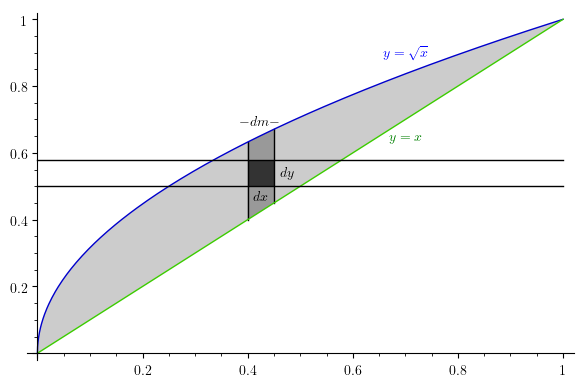
\includegraphics[width=15cm]{qn6.png}
        \centering
    \end{figure}
    Consider a small section of the shape (highlighted in black), with volume = $dx dy T$. It has small mass $ddm=dx dy T \delta(x,y) = dx dy T (1+y)$. To find the mass of thin strip $dm$, one must sum up all the masses of black squares from the top curve to the bottom curve, that is:
    \begin{align}
        dm &= \int^{\sqrt x}_x (1+y) dy dx T \nonumber \\
        &= T dx (y+\frac{1}{2}y^2 \big|^{\sqrt x}_x \nonumber \\
        &= T (\sqrt{x}-\frac{1}{2}x-\frac{1}{2}x^2) dx
    \end{align}
    We can now find $x_{cm}$ in terms of $M$ and $T$.
    \begin{align*}
        x_{cm} &= \frac{1}{M}\int^1_0 x dm \\
        &=\frac{T}{M} \int^1_0 x\sqrt{x} -\frac{1}{2}x^2-\frac{1}{2}x^3 dx \\
        &= \frac{13}{120} \frac{T}{M}
    \end{align*}
    To get rid of the $T/M$ term, note that $M$ is simply the total mass of the object. If we integrated $dm$ from 0 to 1, we would get $M$. Using (5):
    \begin{align*}
        M&=\int^1_0 dm \\
        &=\int^1_0 T (\sqrt{x}-\frac{1}{2}x-\frac{1}{2}x^2) dx \\
        &=T\frac{1}{4}
    \end{align*}
    We have that $M/T=1/4$ and hence $T/M=4$. So $x_{cm} = 13/120 \times 4 = 13/30$.
    
    $y_{cm}$ is a little easier as the density does not vary in a strip. (ie. the density in the piece enclosed by the 2 horizontal lines in the picture above is the same throughout the piece). Dividing the piece into horizontal strips $dm$, to find the mass of a small strip $dm$, one must integrate $ddm$ from $y$ to $y^2$.
    \begin{align*}
        dm &= \int^{y}_{y^2} (1+y) dy dx T\\
        &= T (y -y^3) dy
    \end{align*}
    \begin{align*}
        y_{cm} &= \frac{1}{M}\int^1_0 y dm \\
        &=\frac{T}{M} \int^1_0 y^2-y^4 dy \\
        &= \frac{2}{15} \frac{T}{M} \ \ \text{(From 5)}\\
        &= \frac{8}{15}
    \end{align*}
    Thus the coordinates of the COM are $(x_{cm}, y_{cm})= (13/30, 8/15)$.
\end{enumerate}


\end{document}
